
%~~~~~~~~~~~~~~~~~~~~~~~~~~~~~~~~~~~~~~~~~~~~~~~~~~~~~~~~~~~~~~~~~~~~~~~~~~~~~~~~~~~~~~~~~~~~~~~~~~~~~~~~~~~
% new subsection
%~~~~~~~~~~~~~~~~~~~~~~~~~~~~~~~~~~~~~~~~~~~~~~~~~~~~~~~~~~~~~~~~~~~~~~~~~~~~~~~~~~~~~~~~~~~~~~~~~~~~~~~~~~~
\chapter{Calculating Critical Strain Energy}\label{sec:pebble-crush-prediction}
It is impractical, if not impossible, to experimentally measure accurate contact forces between all the pebbles in a densely-packed, three-dimensional ensemble. In investigating the probability of pebbles becoming damaged (\textit{i.e.} crushed or cracked) in a packed bed, we therefore rely on the combined information gained from indirect measurements of the entire pebble bed, crush experiments of individual pebbles, and the predictive capabilities of DEM simulations. With the rise of micro-mechanical tools and computing power, attempting to predict when ceramic pebbles will crush in an ensemble, based on inter-particle contact forces, has received considerable attention.\cite{Marketos2007,Pitchumani2004} Research on pebble damage has also been taken up by others in the fusion community to predict the onset of pebble crushing as a function of an external pressure and the resulting changes to mechanical properties such as the stress-strain of the pebble bed.\cite{Annabattula2012a, Zhao2012, Zhao2013}

Statistical probability arguments were applied to the study of packed beds of brittle grains by Marketos and Bolton\cite{Marketos2007}. The fundamental assumption in their predictive method was the independence of crushing events. They used their model to predict the initiation of crushing as well as the evolution of the packing after crushing. They created somewhat arbitrary probability distributions of the strength of their granular particles,
\begin{equation}
	h(\Phi) = \frac{0.0395}{\sqrt{\Phi}}
\end{equation}
where $\Phi$ is a characteristic strength parameter falling between 160 and 640~N. The form of their distribution was based on single crushing tests on quartz particles from Nakata\etal.

A common alternative distribution is to use a form first proposed by Weibull for a material under uniform stress\cite{Kwok2013,Zhao2011,nakata1999probabilistic,Zhao2013,Pitchumani2004}. The form, as written by Zhao\etal~is,
\begin{equation}
	P_s = 1 - \exp\left[-\left(\frac{W_c}{W_\text{mat}}\right)^m\right]
\end{equation}
where $W_c$ is the energy absorbed by the pebble and $W_\text{mat}$ and $m$ characterize the material. An important note is how to calculate the critical strain energy for the pebble. Refs.~\cite{Marketos2007} and \cite{Zhao2011} note the necessity to consider the coordination number dependence on total strain energy. In other words, the total strain energy is the cumulative total of strain energy at every contact. Zhao\etal~give the critical strain as
\begin{equation}
	W_c = \sum_{i=1}^{Z}\left(\frac{9}{80 R_{ij}^*}\right)^{1/3} \left(\frac{1}{E_{ij}^*}\right)^{2/3} F_{n,ij}^{5/3}
\end{equation}
where $Z$ is the coordination number of pebble $i$. 

However, Russell\etal, analyzed simple, ideal granular assemblies for which they could find analytical solutions to stress distributions inside of pebbles.\cite{Russell2009} In their work, failure of a granular particle initiates at the location of maximum stress invariant ratios. In the contact of elastic spheres, the stress fields near the contact areas are highly localized. Because of the highly localized effects, Russell\etal~find that in granular assemblies the contributions to failure initiation are not additive. They discovered that the initiation of failure is always located adjacent to the largest force irrespective of the material properties or geometric size of the pebbles in an ensemble. Russell\etal~conclude: \emph{the largest contact force acting upon a particle is the primary agent driving the damage of the individual}.\cite{Russell2009} Based upon the failure criterion developed for brittle materials, crushing of an individual does not directly depend upon the presence or magnitude of any lesser contact forces acting on the particle. Although their results were obtained for idealized assemblies, the results are generally true for any situation where multiple contact forces are present.




Based on the compelling arguments of Russell\etal, I define a pebble in an ensemble to crush \emph{when a single contact force surpasses a defined critical value for that pebble}. The definition of the critical force is an empirical value derived from experiments on single pebbles. Because the normal force between two elastic objects is a function of the material properties of the interacting objects (see, \textit{e.g.}, \Cref{eq:hertz-normal-force}), we cannot directly compare the forces between the pebble and test stand with pebble-pebble contacts in an ensemble. An alternative is to integrate the force along displacement, resulting in strain energy of the contact. The strain energy can then relate the contact forces between different material interactions, in a similar manner to Refs\cite{Zhao2013,Annabattula2012a}.

We begin by integrating the Hertzian force along the overlap of contact to find the strain energy $W_\epsilon$, of contact between any two materials,
\begin{equation}\label{eq:strain-energy-integral}
	W_\epsilon = \int_0^{\delta_c}\!F_n(\delta')\,\mathrm{d}\delta'
\end{equation}
where the upper limit of the integration is the critical overlap $\delta_c$. Inserting the Hertzian relation of \Cref{eq:hertz-normal-force} into \Cref{eq:strain-energy-integral} gives,
\begin{align}
	W_\epsilon& = \int_0^{\delta_c}\!  \frac{4}{3}E^*\sqrt{R^*}\,\delta'^{3/2} \,\mathrm{d}\delta' \\
	%W_\epsilon & = \frac{4}{3}E^*\sqrt{R^*} \left[\frac{2}{5}\,{\delta_c}^{5/2}\right] \\
	W_\epsilon & = \frac{8}{15}E^*\sqrt{R^*}\, {\delta_c}^{5/2}
\end{align}

I will call the strain energy of the pebble compressed between platens as the lab strain energy, $W_{\epsilon,L}$. In pebble crushing experiments, we record the strain energy absorbed up to the point of crushing, the data for \lis~and \lit~pebbles are shown in \Cref{fig:fzk-w-hist} and~\Cref{fig:nfri-w-hist}, respectively. The strain energy of two particles in contact will be the bed strain energy, $W_{\epsilon,B}$. The assumption is made that, if each contact interaction computed in DEM simulations is integrated to the proper critical overlap, the strain energies will be equal at that contact. Thus lab strain energy is equated to bed strain energy to find the critical ensemble overlap value, $\delta_{c,B}$, in terms of experimental values,
\begin{equation}
	W_{\epsilon,L} = W_{\epsilon,B} = \frac{8}{15}E_B^*\sqrt{R_B^*}\, {\delta_{c,B}}^{5/2}
\end{equation}
the critical pebble bed overlap is therefore,
\begin{equation}
	\delta_{c,B} = \left[\frac{15W_{\epsilon,L}}{8E_B^*\sqrt{R_B^*}}\right]^{2/5}
\end{equation}

This overlap can be reinserted to the Hertz force of \Cref{eq:hertz-normal-force} to find the critical force (crush force) of the interacting particles in the numeric ensemble as a function of the critical strain energy of the lab. Doing this, we find,
\begin{equation}\label{eq:peb_hertz}
	F_{c,B} = C{E_B^*}^{2/5}{R_B^*}^{1/5}W_{\epsilon,L}^{3/5}
\end{equation}
where $C = \frac{4}{3}\left(\frac{15}{8}\right)^{3/5}$.
\begin{figure}[ht]
\centering
    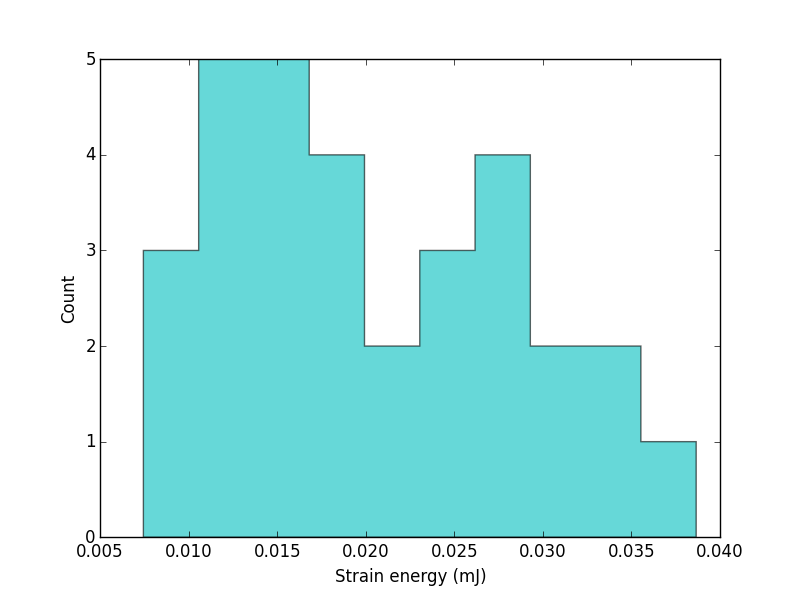
\includegraphics[width=\doubleimagewidth]{figures/fzk-w-histogram.png}
    \caption{Histogram of the absorbed strain energy at the moment of crushing for \lis~pebbles as measured in single pebble crush experiments.}
    \label{fig:fzk-w-hist}
\end{figure}

\begin{figure}
        \centering
        \begin{subfigure}[b]{\doubleimagewidth}
                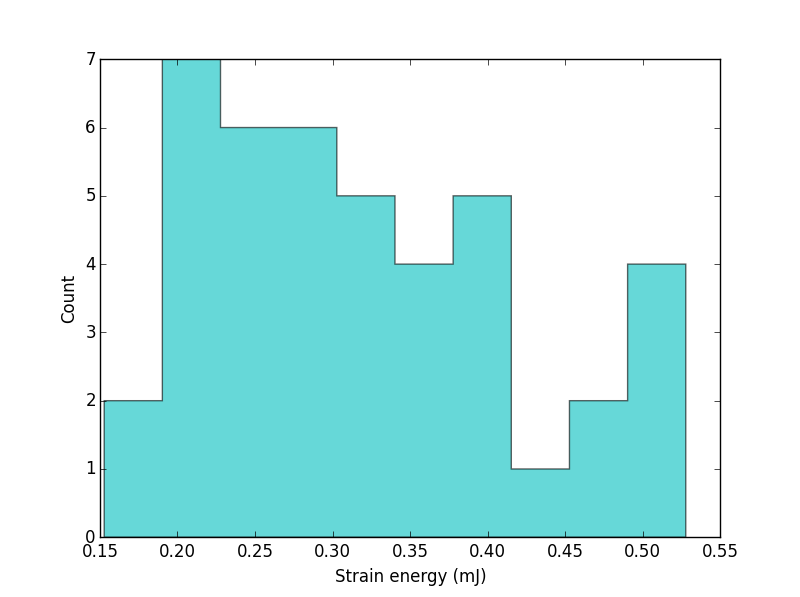
\includegraphics[width=\textwidth]{figures/nfri-1mm-w-histogram.png}
                \caption{$\bar{d}_p = 1$ mm}
                \label{fig:nfri-1-w-hist}
        \end{subfigure}
        ~
        \begin{subfigure}[b]{\doubleimagewidth}
                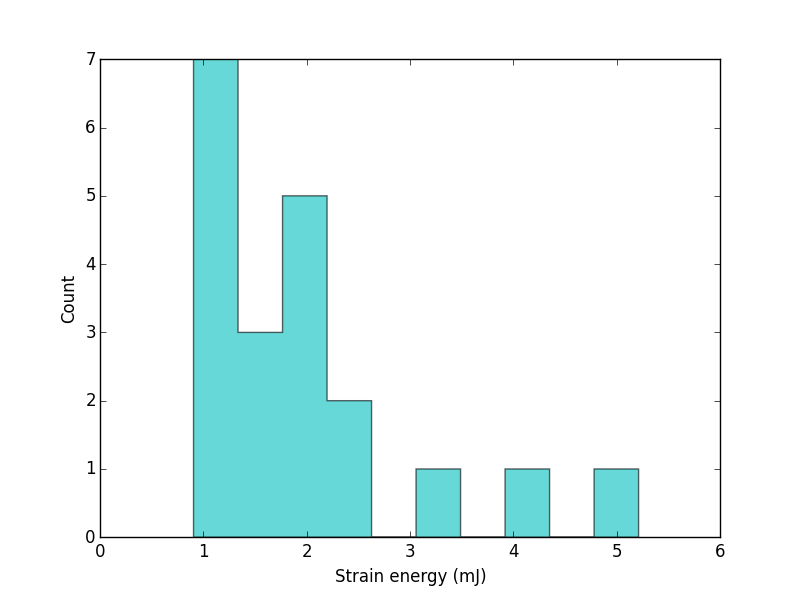
\includegraphics[width=\textwidth]{figures/nfri-1.5mm-w-histogram.png}
                \caption{$\bar{d}_p = 1.5$ mm}
                \label{fig:nfri-1.5-w-hist}
        \end{subfigure}
        \caption{Histogram of the absorbed strain energy at the moment of crushing for \lit~pebbles as measured in single pebble crush experiments.}\label{fig:nfri-w-hist}
\end{figure}

\Cref{eq:peb_hertz} is a generic translation between lab materials and packed bed materials. We will use the equation as the basis for our pebble crushing prediction in DEM simulations. During the DEM run, we can find the maximum normal force acting on each pebble,
\begin{equation}\label{eq:find_fmax}
	F_{c} = \max F_{n,ij}
\end{equation}
We then define in a straightforward way a pebble crushing event as occurring when the pebble's maximum normal force is greater than the critical bed force defined in \Cref{eq:peb_hertz},
\begin{equation}\label{eq:crush-predict}
  F_{c} > F_{c,B} = \frac{4}{3}\left(\frac{15}{8}\right)^{3/5}{E_B^*}^{2/5}{R_B^*}^{1/5}W_{\epsilon,L}^{3/5}
\end{equation}

Example values of critical crush forces, predicted from \Cref{eq:crush-predict} are given in \Cref{fig:crush-force-contours}. From \Cref{sec:exp-reduction-factor}, Young's Modulus was seen to vary widely among tested pebbles; for this calculation a range of \SIrange{10}{100}{\giga\pascal} is used along with a generic Poisson ratio of \num{0.24} for finding $E^*$. A constant pebble radius of $R_p = \SI{0.5}{\milli\meter}$ is used. A large variation of measured strain energy was seen between \lis~and \lit; a range of \SIrange{0.1}{1}{\micro\joule} is chosen for this calculation.

\begin{figure}[ht]
\centering
    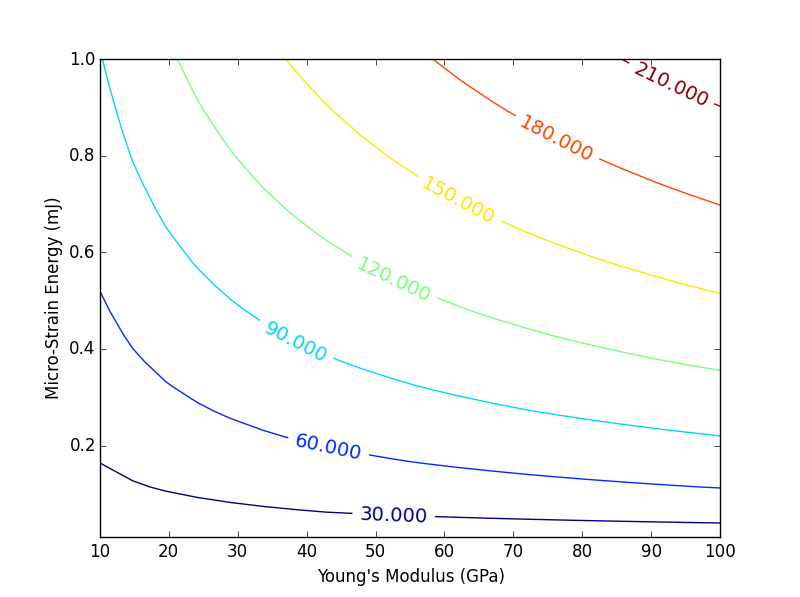
\includegraphics[width=\doubleimagewidth]{figures/crush-force-contours.png}
    \caption{Contour map of critical crush force values as a function of Young's Modulus and micro strain energy.}
    \label{fig:crush-force-contours}
\end{figure}

\FloatBarrier

For implementation in DEM, the crush force prediction becomes probabilistic naturally due to the distribution of strain energies measured in experiments; therefore imparting a distribution shape to the $F_{c,B}$ prediction. Cumulative distribution functions are generated for the experimental strain energy data for which we fit Weibull distribution curves, of the form
\begin{equation}
	\Xi = \lambda\left[-\ln(W_\epsilon)\right]^{1/\sigma}
\end{equation}
where the shape parameter, $\sigma$, is fit to the specific curve of each set of experimental data and the second parameter, $\lambda$ is defined as
\[
\lambda = \bar{W}_\epsilon - \min W_\epsilon
\]
In \Cref{fig:fzk-w-cdf} and~\Cref{fig:nfri-w-cdf} we see the experimental data and the Weibull fits specific to the ceramic material and batch. The figures illustrate goodness of Weibull fits. The Weibull distribution functions are recreated numerically in the assignment of each pebbles `critical bed force' value. 



\begin{figure}[ht]
\centering
    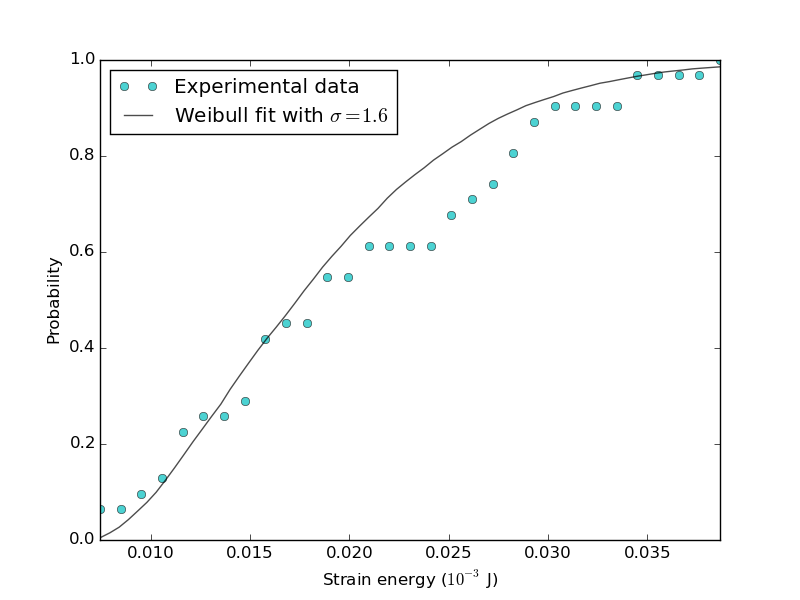
\includegraphics[width=\doubleimagewidth]{figures/fzk-w-cdf-fit.png}
    \caption{Cumulative distribution function for strain energy with a Weibull distribution fit with shape parameter specific for the \lis~pebbles. The shape parameters are used in numeric replications.}
    \label{fig:fzk-w-cdf}
\end{figure}

\begin{figure}
        \centering
        \begin{subfigure}[b]{\doubleimagewidth}
                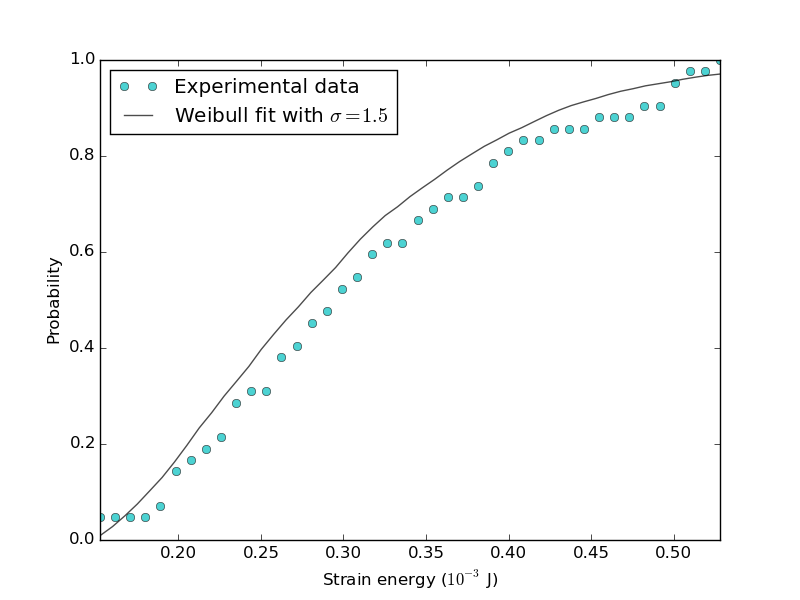
\includegraphics[width=\textwidth]{figures/nfri-1mm-w-cdf-fit.png}
                \caption{$\bar{d}_p = 1$ mm}
                \label{fig:nfri-1-w-cdf}
        \end{subfigure}
        ~
        \begin{subfigure}[b]{\doubleimagewidth}
                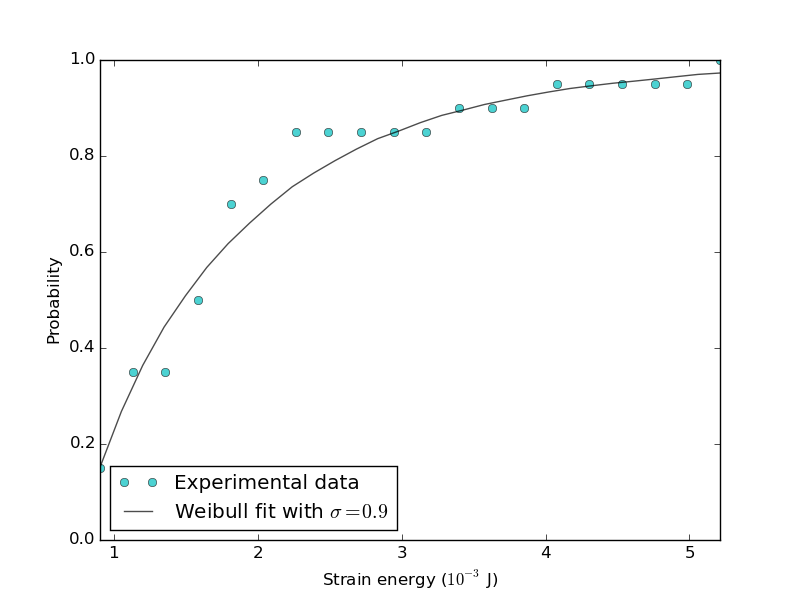
\includegraphics[width=\textwidth]{figures/nfri-1.5mm-w-cdf-fit.png}
                \caption{$\bar{d}_p = 1.5$ mm}
                \label{fig:nfri-1.5-w-cdf}
        \end{subfigure}
        \caption{Cumulative distribution function for strain energy with a Weibull distribution fit with shape parameter specific for the two batches of \lit~pebbles. The shape parameters are used in numeric replications.}\label{fig:nfri-w-cdf}
\end{figure}



In this section we have proposed a numerical basis for predicting pebble crushing in a ceramic pebble bed based on translations of strain energy distribution functions of experimental data. Implementation in DEM simulations requires defining an array of strain energies, the distribution of which must satisfy Weibull distributions matching experimental data for the specific pebble under consideration. The array of strain energies is loaded as a dictionary variable with the DEM pebble identification number as key and strain energy as value. Then we loop through all pebble IDs in the ensemble and check the criteria defined in \Cref{eq:crush-predict}. If a pebble's maximum force exceeds the crush criteria, the pebble is flagged for fragmentation. Similar to implementation of thermal expansion, it is possible at every time step to check for broken pebbles. However, the stress on pebbles is due to thermal expansion and is therefore nonsensical to check for broken pebbles more frequently than updating pebble diameters with thermal expansion; therefore the same timestep is used in both of these custom numerical routines. 

The equations established here present the framework for implementing crush prediction in DEM models. However, there is currently no experimental data with which to validate or calibrate the model. A parametric study of pebble crushing in uniaxial compression tests could be performed, as has been done by others (See Refs.\cite{Annabattula2012a,Zhao2013}). But without necessary experimental data, the impact of their results is also somewhat lacking.

When a pebble has been flagged as being crushed, it is quite another task to model the fragmentation. Many researchers have made attempts at implementing various tricks to attempt to capture the effects of pebbles crushing in an ensemble. In the next section I will review some of the past efforts as well as a new approach and some evaluation of the work.